\chapter{Density Functional Theory}
Переважна теоретична картина твердотільних та / або молекулярних систем включає неоднорідний електронний газ: набір взаємодіючих точкових електронів, що рухаються квантово-механічно в потенційному полі набору атомів, які вважаються статичними (наближення Борна–Оппенгеймера). Рішення таких моделей зазвичай вимагає використання схем апроксимації, з яких найбільш основновною являється апроксимація незалежних електронів, теорія Хартрі і теорія Хартрі–Фока — зазвичай викладаються студентам на курсах фізики і хімії. Однак існує інший підхід-теорія функціоналу щільності (DFT), яка за останні тридцять років або близько того все частіше стає методом який обирають для вирішення завдань розрахунку багаточастинкових систем. Цей метод має подвійну перевагу: він дозволяє вирішувати багато завдань з досить високою точністю, а також є простим в обчислювальному відношенні (простіше навіть, ніж схема Хартрі). Незважаючи на ці переваги, він відсутній у більшості програм бакалаврату та багатьох програм магістратури, з якими ми знайомі.
\section{Загальна теорія}
У цьому розділі представлено єдине трактування термодинаміки і теорії функціоналу щільності. Для простоти спочатку буде розглянуто випадок класичної взаємодіючої системи точкових частинок. Читачеві рекомендується мати на увазі електронні системи, які будуть предметом наступного розділу. Таким чином, рів. \ref{eqn:Ham_}--\ref{eqn:free_energ_functional}, які будуть виведені тут з використанням класичних позначень, в рівній мірі застосовні до квантово-механічних систем, де гільбертовий простір з його операторами положення і імпульсу замінює класичний фазовий простір і його скалярні координати.
\subsection{Термодинаміка}
Ми розпочнемо з переосмислення рівнянь термодинаміки в застосунку до квантовомеханічних систем. Спочатку розглянемо класичну систему з N взаємодіючих частинок в об'ємі V. Гамільтоніан такої системи буде наступним:
\begin{equation}
\label{eqn:Ham_}
	{\cal H}_{mb} = {\cal T} + {\cal U},
\end{equation}
де ${\cal T} = \sum\limits_{i}\textbf{p}_i^2/2m$ -- кінетична енергія $i$-тої частинки та ${\cal U} = \sum_{i < j}u(|\textbf{r}_i - \textbf{r}_j|)$ -- енергія взаємодії у вигляді простого парного потенціалу $u(r)$. Тут $\textbf{p}_i$ та $\textbf{r}_i$ -- координата та імпульс у просторі, $m$ -- її маса. 
Ми розглянемо великий конанічний ансамбль, де система знаходиться у контакті з джерелом тепла з температурою $T$ і з частинковим резервуаром з хімічним потенціалом $\mu$. Як вже відомо з статистичної фізики потенціал вільної енергії у даному випадку задається наступним чином:

\begin{equation}
\label{eqn:omegapotential}
	\Omega(\mu,T,V) = -T\log\Xi,
\end{equation}
 
де $\Xi$ функція омега-розподілу:

\begin{equation}
\label{eqn:sgranddistr}
	\Xi(\mu, T, V) = \sum\limits_{M = 0}^\infty\frac{1}{M!}Tr\exp{\left(-\frac{{\cal H}_{mb} - {\mu} M}{T}\right)},
\end{equation}

температура вказана в одиницях енергії (тобто $k_{B} = 1$), а класичний слід, $Tr$, представляє $6M$-мірний інтеграл по фазовому простору (поділ на $M!$ компенсує подвійний підрахунок станів багатьох тіл нерозрізнених частинок). 

З цих визначень безпосередньо випливає, що математичне очікування числа частинок в системі задається похідною від омега-потенціалу, $N = \langle M \rangle = -(\partial{\Omega}/\partial{\mu})$. Опуклість термодинамічного потенціалу \cite{convexfreeenerg} дає, що $N$ являється функцією $\mu$. Інші часткові похідні $\Omega$ дають значення додаткових фізичних величин, таких як ентропія $S$ та тиск $P$ це може бути узагальнено таким чином $d\Omega = -Nd\mu - SdT - PdV$

В різних контекстах ми повинні використовувати різні ансамблі. Наприклад, при досліджені системи в якій кількість частинок постійна, а хімічний потенціал ні, то краще використовувати вільну енергію Геймгольца, яку можна отримати з омега-потенціалу $\Omega$ за допомогою перетворення Лежандра: $F(N,T,V) = \Omega(\mu(N),T,V)+\mu(N)N.$
Тут $\mu(N)$ більше не являється незалежною змінною, але функція N отримується за допопмогою інвертування співвідношення $N = N({\mu},T,V)=\dfrac{\partial\Omega}{\partial\mu}.$ Похідна $F$ по відношеню до "нової" вільної змінної $N$ дорівнює до "старої" змінної $\mu$. Інші похідні змінних не змінюються. Тому ми можемо записати наступне $dF={\mu}dN - SdT - PdV$.

Для порівняння з DFT буде корисно зробити зробити варіацію обратного перетворення Лежандра, яке виражає потенційну енергію $\Omega$ у термінах вільної енергії $F$ і визначемо наступну омега-потенційну функцію, якак залежить явно від $\mu$ та $N$:
\begin{equation}
	\label{eqn:grand-potentialfunc}
	\Omega_\mu \equiv F(N,T,V) - {\mu} N
\end{equation}
Ця функія дає початковий омега-потенціал рівняння \ref{eqn:omegapotential} при мінімізації відносно $N$, тобто коли похідна $(\partial{F}/\partial{N}) - \mu$ зникає, що еквівалентно умові $N = N(\mu,T,V)$ за звічаї, яке використовується у обратному перетворені Лежандра. Для геометричної інтерпрітації перетвореня Лежандра дивіться рис. \ref{fig:legander_transform}
\begin{figure}[H]
  \centering
  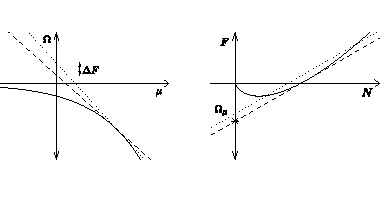
\includegraphics[scale=2.5]{img/Legender_transform.pdf}
  \caption{(a) Перетворення Лежандра, яке дає $F(N)$, відповідає опису кривої $\Omega\mu$ властивостями її дотичних: мінус їх нахили $N = -(\partial{\Omega}/\partial{\mu})$. та їх перетину з енергетичної віссю, $F = \Omega + \mu N$. Той факт, що похідна $\Delta F / \Delta N$ дорівнює $\mu$, слідує з постановки питання: якщо дві сусідні прямі перетинають енергетичну вісь на відстані $\Delta F$ один від одного і мають нахили, які відрізняються на $\Delta N$, на якій відстані від осі вони будуть перетинати один одного? (b) Зворотне перетворення Лежандра з $F(N)$ в $\Omega (\mu)$ має аналогічну інтерпретацію. Мінімізація, запропонована в рівнянні. \ref{eqn:grand-potentialfunc} відповідає вивченню сімейства ліній з фіксованим нахилом $\mu$, які проходять через точки $N, F$ на кривій вільної енергії. Їх перетин, має мінімум (зазначений зірочкою) для тієї лінії, яка є дотичною до кривої.}
  \label{fig:legander_transform}
\end{figure}
\subsection{Підхід Кона-Шема}
Наведене вище обговорення можна досить просто узагальнити на обробку частинок у зовнішньому потенціалі $v(\textbf{r})$. Гамільтоніан багатьох тіл тепер дорівнює
\begin{equation}
\label{eqn:Ham}
	{\cal H}_{mb} = {\cal T} +{\cal V} +{\cal U},
\end{equation}
де ${\cal V} = \sum\limits_{i=0}^M v(\textbf{r}_i)$ -- потенційна енергія. Омега-потенціал і омега-функція були визначені як рів.\ref{eqn:omegapotential} та \ref{eqn:grand-potentialfunc}, але зараз вони залежать від потенціальної функції $v(\textbf{r})$, а не сколярного об'єму $V$. Тому $\Omega = \Omega(\mu, T, [v(\textbf{r})]))$ тепер є функціоналом $v(\textbf{r})$, а тако ж функцією $\mu$ і $T$ -- квадратні дужки позначають функціональні змінні. 

Як добре відомо, потенціал $v(\textbf{r})$ - це енергія, яка вимірюється з довільного джерела, тобто Зміщення потенціалу на постійну величину не впливає на фізику системи. Тут зручно встановити цей початок координат в хімічному потенціалі, тобто прийняти $\mu = 0$. Еквівалентно, можна визначити нову функціональну змінну як $v(\textbf{r}) - \mu$, оскільки $\Omega$ залежить тільки від цієї різниці, а не від $v(\textbf{r})$ і $\mu$ окремо.

Функціональна похідна $\Omega$ за новою змінною дає розподіл щільності частинок, $n(\textbf{r}) = \langle \rho (\textbf{r}) \rangle$, де $\rho(\textbf{r}) = \sum\limits_{i=1}^M\delta(\textbf{r}-\textbf{r}_i)$ неперевірена щільність. Використовуючи (функціональне) перетворення Лежандра, як зазначено вище, ми можемо визначити нову вільну енергію, яка залежить від $n(\textbf{r})$, а не від $v(\textbf{r})$, і називається вільною енергією Хоенберга-Кона:
\begin{equation}
	\label{eqn:free_energ_hoenberg-khon}
	F_{HK}[n(\textbf{r})] = \Omega[v(\textbf{r})] - \int{n(\textbf{r}) v(\textbf{r})d\textbf{r}} 
\end{equation}
де зміною температури у явному вигляді ми знехтували і $v(\textbf{r)}$ з правої частини обрана так, щоб відповідати заданому $n(\textbf{r})$ (такий вибір можливий лише із-за загальної опуклості вільної енергії). Частина та функціональна похідна $F_{HK}[n(\textbf{r})]$ задається звичайним правилом перетворення Лежандра, як: $dF_{HK} = -SdT - \int{v(\textbf{r})\delta n(\textbf{r})d\textbf{r}}$.
Пряме узагальнення функції вильної енергії це і є функціонал вільної енергії:
\begin{equation}
	\label{eqn:free_energ_functional}
	\Omega[n(\textbf{r})] \equiv F_{HK}[n(\textbf{r})] + \int{n(\textbf{r})v(\textbf{r})d\textbf{r}}
\end{equation}
Якщо цей функціонал мінімізувати відносно $n(\textbf{r})$ і при постійному $v(\textbf{r})$ то функціонал вільної енергії дорівнює омега-потенціалу. Існування функціоналу $n(\textbf{r})$ з цією властивістю є одним з основних принципів DFT і є другою теоремою Хоенберга–Кона (див. наступний параграф).

Обговорення теореми Хоенберга-Кона, тим не менш, важливо навіть у введенні до DFT на основі перетворення Лежандра, оскільки процедура мінімізації вільної енергії, втілена в ньому, є центральною як для формування фізичної інтуїтивної картини DFT, так і для розробки ефективних чисельних схем для вирішення рівнянь DFT в практиці.

Узагальніючи можна сказати, що в ТФГ Кона-Шема всі обмінні та кореляційні ефекти включені в обмінно-кореляційний функціонал $E_{xc}[n]$, котрий залежить від густини $n(\textbf{r})$ електронів. 


Функціонал повної енергії може бути записаний, як~\cite{K-S energy}:
\begin{eqnarray}
 E[\psi_i] = 2\sum\limits_{i}\int\psi_i\left({{\hbar^2}\over{2m}}\right)\nabla^2\psi_id^3\textbf{r}+\int V_{ion}(\textbf{r})n(\textbf{r})d^3\textbf{r}+\nonumber \\
 {{e^2}\over{2}}\int {{n(\textbf{r})n(\textbf{r})}\over{|\textbf{r}-\textbf{r}^\prime|}}d^3\textbf{r}d^3\textbf{r}^\prime+E_{xc}[n(\textbf{r}^\prime)]+E_{ion}(R_i)
\end{eqnarray}

Де $V_{ion}$ -- повний електрон-іонний потенціал, $E_{xc}[n(\textbf{r}^\prime)]$ -- обмінно-кореляційний функціонал, $E_{ion}$ -- кулонівська енергія, $n(\textbf{r})$ -- електронна густина

\section{Теореми Кона-Шема}
Шляхом публікації двох статей Хохенбергом та Коном у 1964 році~\cite{Hohenberg&Khon}, а також Коном і Шемом в 1965 році~\cite{Khon&Sham}, в яких доказувались теореми завдяки яким теорія функціоналу ґустини вийшла на новий рівень. Ці теореми встановлюють точну відповідність між електронною щільністю, зовнішнім потенціалом і хвильовою функцією.

\textbf{Перша теорема} говорить про те, що електронна щільність єдиним чином визначає оператор Гамільтона і, отже, всі характеристики системи.
Не можуть існувати два різні зовнішні потенціали, що призводять до однієї і тієї ж електронної щільності основного стану системи, іншими словами, електронна щільність основного стану однозначно визначається зовнішнім потенціалом.
Знаючи потенціал, ми знаємо Гамільтоніан системи, відповідно можемо знайти хвильову функцію системи та всі властивості системи, що визначаються електронною щільністю основного стану. Перша теорема показує зв'язок між зовнішнім потенціалом та електронною щільністю основного стану.

\textbf{Друга теорема} функціонал енергії, що визначає енергію квантового стану системи, визначає мінімальну енергію тоді і тільки тоді, коли електронна густина, що входить у функціонал, є реальною густиною основного квантового стану.
Таким чином, для знаходження точної енергії основного стану та його щільності, достатньо знати функціонал $E[n]$. Висновки цих теорем призводять до того, що для будь-якого зовнішнього потенціалу завжди можна знайти електронну густину та енергію основного стану, мінімізуючи цей функціонал.


\subsection{Самоузгоджене рівняння Кона-Шема}
Електронна щільність системи може бути знайдена з рішення самоузгодженого рівняння Кона-Шема, це випливає з наведених раніше теорем, яке можна записати так:

\begin{equation}
    \left[{{-\hbar^2}\over{2m}}\nabla^2+V_{ion}(\textbf{r})+V_H(\textbf{r})+V_{XC}(\textbf{r})\right]\psi_i(\textbf{r}) = e_i\psi_i(\textbf{r})
\end{equation}

Де $\psi_i$ -- хвильова функція стану $i$, $e_i$ -- власні значення, $V_H$ -- потенціал Хартирі, який відповідає за електронно-електронне відштовхування.

Явний вид обмінно-кореляційного потенціалу $V_{XC}$ ми не можемо знати принципово, тому його задають формально, функціональною похідною: 

\begin{equation}
    V_{XC} = \frac{\partial E_{XC}[n(\textbf{r})]}{\partial n(\textbf{r})}
\end{equation}

Для визначення об'ємно-кореляційного потенціалу використовують ряд наближень, про які ми поговоримо у наступному розділі.


\section{Методи апроксимації \textbf{$E_{xc}$}}
\subsection{LDA}
LDA (local density approximation) -- це клас наближень для обмінно-кореляційної енергії $E_{XC}$ у ТФГ, яка залежить виключно від електронної густини в кожній точці простору. Найуспішнішими локальними наближеннями є ті, що були отримані з моделі однорідного електронного газу (HEG)~\cite{Hohenberg&Khon}. 

Можна записати наступний вираз для обмінно-кореляційної енергії:

\begin{equation}
    E_{XC}^{LDA}[n(\textbf{r})] = \int{\epsilon_{xc}[n(\textbf{r})]n(\textbf{r})d^3\textbf{r}}
\end{equation}

Існує ряд параметрів для LDA, але ми їх не розглядатимемо.

\subsection{GGA}
GGA (generalized gradient approximations) -- на відміну від LDA в даний клас наближень включено градієнтну поправку для електронної щільності. Це усуває деякі недоліки LDA. Для узагальненого градієнтного наближення ми можемо записати, що $E_{xc}$ дорівнює деякій функції локальної щільності та її градієнта:

\begin{equation}
    E_{xc}^{GGA} = \int{f[n(\textbf{r}),\nabla{n(\textbf{r})]n(\textbf{r})d^3\textbf{r}}}
\end{equation}

Найчастіше для розрахунків використовуються параметризації PBE (Perdew-Burke-Ernzerhof)~\cite{PBE} та PW91~\cite{PW91}.

\subsection{meta-GGA}
Фактично meta-GGA - це розширене наближення GGA. В яке, як вхідні дані, входить щільність позитивної орбітальної кінетичної енергії~\cite{Swapan&Gosh&Parr, Becke&Roussel, Tao&Perdew}.

У напівлокальному наближенні функціонал $E_{xc}$ зводиться до єдиного інтегралу загального вигляду:
\begin{equation}
    E_{XC}^{MGGA} = \int{\epsilon_{xc}[n(\textbf{r}),\nabla{n(\textbf{r}),\tau_{\sigma}(\textbf{r}})]}n(\textbf{r})d^3\textbf{r}
\end{equation}

Де $\tau_{\sigma}(\textbf{r})$ щільність кінетичної енергії зайнятих станів та визначається як:
\begin{equation}
    \tau_{\sigma}(\textbf{r}) = \sum\limits_{i\textbf{k}}|\nabla\psi_{i\textbf{k}}(\textbf{r})|^2
\end{equation}
\subsubsection{SCAN}
SCAN (Strongly-constrained and appropriately-normed) meta-GGA, раніше розроблені meta-GGA функціонали виявилися менш точними для розрахунку критичних тисків у структурно-фазових переходах твердих тіл, а також для матеріалів з шаруватою структурою відомі, як Ван-дер-Ваальсовські матеріали. SCAN покликаний усунути цю проблему за допомогою додавання в обмінно-кореляційний функціонал безрозмірну змінну.
$\alpha$~\cite{SCAN}:
\begin{equation}
	\label{eqn:alpha}
    \alpha = (\tau - \tau^W)/\tau^{unif} > 0
\end{equation}

Де $\tau^W = |\nabla{n(\textbf{r})}|^2/8n(\textbf{r})$ є одноорбітальною межею $\tau$ \newline та $\tau^{unif} = (3/10)(3\pi^2)^{2/3}n(\textbf{r})^{5/3}$ межа рівномірної щільності.

Відомі багато особливостей точного функціоналу $E_{xc}$. неемпіричні функціонали, побудовані для задоволення точних обмежень на цей функціонал щільності, надійні в широкому діапазоні систем (наприклад, атомів, молекул, твердих тіл і поверхонь), включаючи багато, які не схожі на ті, для яких ці функціонали були протестовані і підтверджені. У цьому розділі ми більш глибше розкриємо імплементацію фукнкціоналу, який вперше задовольняє всім відомим можливим точним обмеженням[ADD LIST] і відповідним чином нормується в системах, для яких напівлокальні функціонали можуть бути точними або надзвичайно точними.

Запишемо кореляційну енергію $\epsilon_c$ на один електрон \ref{eqn:e_c}. Також намалюємо "correlation enhancement factor" $F_{xc}(r_s, \xi, s, a)$ в наближені низької густини $r_s \rightarrow \infty$ [ADD GRAPH] та інтерполяційну/екстрополяційну функцію $f_x(a)$ та $f_c(a)$. Тут $\xi = (n_\uparrow - n_\downarrow)/(n_\uparrow + n_\downarrow)$ спін полярізація, $r_s = (4 \pi n/3)^{-1/3}$, і $s = {|\nabla{n}|}/{2(3\pi^2)^{-1/3}n^{4/3}}$, $\alpha$ -- безрозмірний параметр \ref{eqn:alpha}. 

Полулокальний обмінно-корелляційний функціонал можно записати наступним чином (знехтуємо $\nabla \xi$ та припустимо що параметр $\alpha$ однаковий для спін-непарлезаціних густин $2n_\uparrow$ та $2n_\downarrow$):
\begin{equation}
	\label{eqn:semilocalexc}
	E_{xc}[n_{\uparrow},n_{\downarrow}] = \int{d^3 r n\epsilon_{xc} = \int d^3 r n \epsilon_{x}(n)F(r_s,\xi, s, a)}
\end{equation}
Де $\epsilon_x^{unif} = -(3/4\pi)(3\pi^2n)^{1/3}$ обмінна енергія на електрон однорідного електроного газу.  
Корелляційну частину можна записати як: 

\begin{equation}
	\label{eqn:cor}
	E_{c}[n\uparrow,n\downarrow] = \int{d^3 n \epsilon_c (r_s,\xi, s, a)}
\end{equation}
SCAN $\epsilon_c$ має наступну форму:
\begin{equation}
	\label{eqn:e_c}
	\epsilon_c = \epsilon_c^1 + f_c(\alpha)(\epsilon_c^0 -\epsilon_c^1)
\end{equation}

\subsubsection{SCAN+rVV10}
Складність опису "шаруватих" матеріалів виникає через нелокальну далекодійну природу ван дер Ваальсовської взаємодії, а також через її більш слабкий зв'язок в порівнянні з хімічною. Повний облік взаємодії Ван дер Ваальса досягається такими дорогими методами, як Монте Карло (QMC)~\cite{QMC}, одиничні та подвійні зв'язані кластери з перетурбованими трійками (CCSD(T))~\cite{CCSD(T)} та інші, через їхню дорожнечу їх використовують тільки на строго обмежених системах. Поправка rVV10 має такі параметри як $b$, який відповідає за короткодійну поведінку нелокальної кореляційної енергії, а також $C$, що відповідає за так звану локальну заборонену зону. Ці параметри фітуються на S22. Набір даних тесту S22~\cite{S22} використовується для оцінки відносної точності методів vdW-DF, також обговорюються такі фактори, як масштабованість та переносність.